\documentclass[a4paper, 12pt]{article}%тип документа

%%%Библиотеки
	%\usepackage[warn]{mathtext}	
	\usepackage[T2A]{fontenc} % кодировка
	\usepackage[utf8]{inputenc} % кодировка исходного текста
	\usepackage[english,russian]{babel} % локализация и переносы
	\usepackage{caption}
	\usepackage{listings}
	\usepackage{amsmath,amsfonts,amssymb,amsthm,mathtools}
	\usepackage{wasysym}
	\usepackage{graphicx}%Вставка картинок правильная
	\usepackage{float}%"Плавающие" картинки
	\usepackage{wrapfig}%Обтекание фигур (таблиц, картинок и прочего)
	\usepackage{fancyhdr} %загрузим пакет
	\usepackage{lscape}
	\usepackage{xcolor}
	\usepackage[normalem]{ulem}
	\usepackage{hyperref}

%%%Конец библиотек




%%%Настройка ссылок
	\hypersetup
	{
		colorlinks=true,
		linkcolor=blue,
		filecolor=magenta,
		urlcolor=blue
	}
%%%Конец настройки ссылок


%%%Настройка колонтитулы
	\pagestyle{fancy}
	\fancyhead{}
	\fancyhead[L]{Лабораторная работа}
	\fancyhead[R]{Талашкевич Даниил, группа Б01-008}
	\fancyfoot[C]{\thepage}
%%%конец настройки колонтитулы



							\begin{document}
						%%%%Начало документа%%%%


%%%Начало титульника
\begin{titlepage}

	\newpage
	\begin{center}
		\normalsize Московский физико-технический институт \\(госудраственный 			университет)
	\end{center}

	\vspace{6em}

	\begin{center}
		\Large Лабораторная работа по квантовой физике\\
	\end{center}

	\vspace{1em}

	\begin{center}
		\large \textbf{Тепловое излучение [8.1]}
	\end{center}

	\vspace{2em}

	\begin{center}
		\large Талашкевич Даниил Александрович\\
		Группа Б01-008
	\end{center}

	\vspace{\fill}

	\begin{center}
	Долгопрудный \\2022
	\end{center}
	
\end{titlepage}
%%%Конец Титульника



%%%Настройка оглавления и нумерации страниц
	\thispagestyle{empty}
	\newpage
	\tableofcontents
	\newpage
	\setcounter{page}{1}
%%%Настройка оглавления и нумерации страниц


					%%%%%%Начало работы с текстом%%%%%%


\section{Аннотация}

\ \ \ \ \textbf{Цель работы:} При помощи модели абсолютно чёрного тела проведение измерения температуры оптическим пирометром с исчезающей нитью и термопарой; Исследование излучение накалённых тел с различной испускательной способностью; Определение постоянных Планка и Стефана-Больцмана

\textbf{В работе используются:} оптический пирометр, модель абсолютно чёрного тела, образцы колец, вольфрамовая лампа, неоновая лампа, блок питания, цифровые вольтметры

\section{Теоретические положения}
Для измерения температуры разогретых тел, удалённых от наблюдателя, применяют методы оптической пирометрии, основанные на использовании зависимости испускательной способности исследуемого тела от температуры. Различают три температуры, функционально связанные с истинной термодинамической температурой и излучательной способностью тела: радиационную $T_{rad}$, цветовую $T_{col}$ и яркостную $T_{b_r}$. \par
В работе измеряется яркостная температура. \textbf{Яркостная температура} - это температура абсолютно чёрного тела, при которой его спектральная испускательная способность равна спектральной испускательной способности исследуемого тела при той же длине волны.
 Измерение яркостной температуры раскалённого тела производится при помощи оптического пирометра с исчезающей нитью, основанного на визуальном сравнении яркости раскалённой нити с яркостью изображения исследуемого тела. \par
Яркостная температура тела всегда ниже его термодинамической температуры. Это связано с тем, что любое нечёрное тело излучает меньше, чем АЧТ при той же температуре. Зависимость между яркостной и термодинамической температурами вольфрама приведена на рис. 1

\begin{figure}[!h]
    \centering
    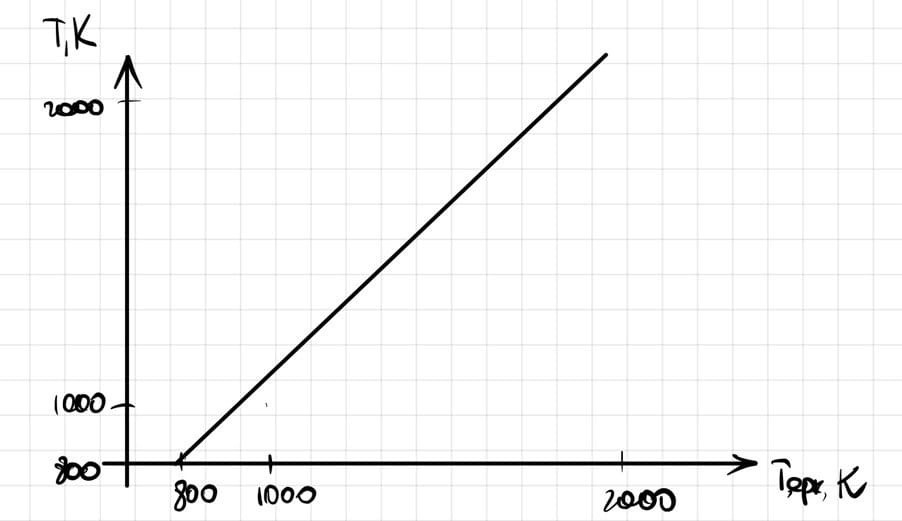
\includegraphics[width=10cm]{fig1.png}
    \caption{График зависимости $T = f(T_{b_r})$ для вольфрам}
    \label{fig:vac}
\end{figure}

По результатам измерений мощности излучения вольфрамовой нити можно судить о справедливости закона Стефана-Больцмана. Если бы нить излучала как АЧТ, то баланс потребляемой и излучаемой энергии определялся бы соотношением 
\begin{equation}
    W = \sigma S (T^4 - T_0^4),
\end{equation}
где $W$ - потребляемая нитью электрическая мощность, $S$ - площадь излучающей поверхности нити, $T$ - температура нити, $T_0$ - температура окружающей среды. Однако вольфрамовая нить излучает как серое тел, и излучение её ослаблено по сравнению с АЧТ в $\varepsilon_T$ раз для любой волны при данной температуре тела Т. Тогда предположив, что нить излучает как серое тело и с учётом того, что $T_0 \ll T$, выражение (1) можно переписать в виде
\begin{equation}
    W = \varepsilon_T S \sigma T^4
\end{equation}
В справедливости закона Стефана-Больцмана можно убедиться, построив график зависимости $W(T)$ в логарифмическом масштабе и по углу наклона определить показатель степени $n$ исследуемой температурной зависимости. В пределах погрешности показатель степени должен быть близок к четырём. \par
Также из формулы (2) можно определить постоянную Стефана-Больцмана.

\section{Экспериментальная установка}

\begin{figure}[!h]
    \centering
    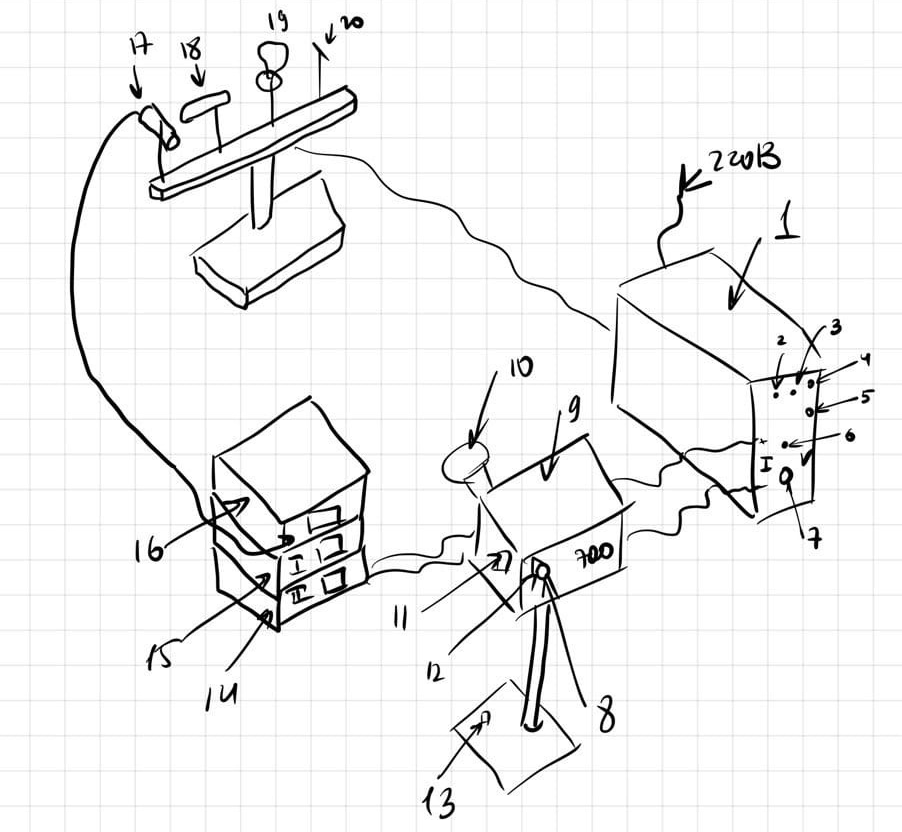
\includegraphics[width=11cm]{fig2.png}
    \caption{Схема экспериментальной установки: 1 - блок питания; 2 - тумблер включения питания образцов; 3 - тумблер нагрева нити пирометра; 4 - кнопка "Нагрев нити"; 5 - кнопка "охлаждение нити"; 6 - тумблер переключения образцов; 7 - регулятор мощности нагрева образцов; 8 - окуляр пирометра; 9 - корпус пирометра; 10 - объектив пирометра; 11 - переключение диапазонов; 12 - ручка смещения красного светофильтра; 13 - регулировочный винт; 14 - вольтметр (напряжение на лампе накаливания); 15 - амперметр (ток через образцы); 16 - вольтметр в цепи термопары; 17 - модель АЧТ; 18 трубка с кольцами из материалов с различной излучательной способностью; 19 - лампа накаливания; 20 - неоновая лампочка}
    \label{fig:vac}
\end{figure}

Исследуемые в работе образцы:
\begin{itemize}
    \item \textbf{модель абсолютно чёрного тела} - керамическая трубка, закрытая с одного конца и окружённая для теплоизоляции внешним кожухом. Температура в трубке измеряется с помощью термопары хромель-алюмель
    \item \textbf{керамическая трубка с набором колец из различных материалов}, нагреваемая изнутри нихромовой спиралью. Материалы колец имеют различную излучательную способность
    \item \textbf{вольфрамовая нить электрической лампочки}
\end{itemize}


\section{Ход работы}

\subsection{Изучение работы оптического пирометра}

    Цель пункта: помощью пирометра измеряется температура модели АЧТ и проводится сравнение её значения со значением температуры, измеренной при помощи термопарного термометра.

\begin{enumerate}
    \item Настроим пирометр, прогреем его нить. Прогреем модель АЧТ.
    \item Введём красный светофильтр пирометра. Изменяя ток через нить пирометра, добьёмся исчезновения нити на фоне изображения раскалённой поверхности дна АЧТ.

    \begin{table}[h]
        \centering
        \begin{center}
            \caption{Сравнение температур АЧТ, выдаваемое пирометром и измеренное термпопарой}
        \end{center}
        \begin{tabular}{|l|l|l|l|l|l|l|}
        \hline
        $T$, $^\circ C$ (убывание)          & 936  & 936 & 931 & 934 & $\langle T \rangle $, $^\circ C$ & $934 \pm 5$  \\ \cline{1-5} \cline{7-7} 
        $T$, $^\circ C$ (возрастание)       & 928  & 927 & 931 & 933 & $\langle T \rangle $, $^\circ C$ & $930 \pm 5$ \\ \hline
        $V$, мВ                            & \multicolumn{4}{l|}{37,41} & $T_{\text{термопара}}$, $^\circ C$              & $938 \pm 2$        \\ \hline
        \end{tabular}
        \label{table:comparison}
    \end{table}

\end{enumerate}

    Из таблицы следует, что пирометр проградуирован по АЧТ точно в пределах погрешностей измерений.

\subsection{Измерение яркостной температуры накалённых тел}

    При нагревании керамической трубки с помощтю пирометра зафиксировано, что различные кольца обладают различными яркостными температурами вследствие различяи спектральных светимостей. Яркостные температуры тел измерить не удалось из-за того, что свечения колец оказалось достаточно слабым (невозможно определить, одинаковы ли яркости нити и кольца).

\subsection{Проверка закона Стефана-Больцмана}

    Нагреем лампу накаливания ло тёмно-красного свечения, а затем будем увеличивать её температуру, снимая значения силы тока и напряжения на лампе. Измеренная яркостная температура преобразуется в термодинамическую температуру с помощью графика завивимости $T(T_{\text{ярк}})$. 

    Закон Стефана-Больцмана в случае вольфрамовой лампы накаливания для проверки имеет вид
    \begin{equation}
        W = \varepsilon_T S \sigma T^n \Rightarrow \ln W = \ln (\varepsilon_T S \sigma) + n \ln T,
    \end{equation}
    или
    \begin{equation}
        \ln W - \ln (\varepsilon_T S \sigma) = n \ln T,
    \end{equation}
    где $\varepsilon_T = \varepsilon_T (T)$, зависимость представлена в виде таблицы для различных температур вольфрама, а $S = \; 5 \text{см}^2$ -- площадь поверхностей нитей накаливания.

    \begin{figure}[h!]
        \centering
        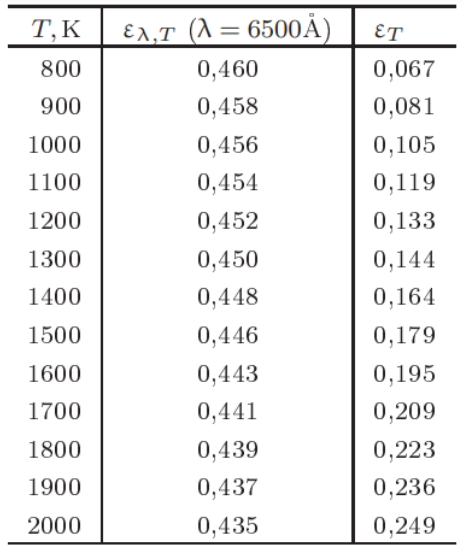
\includegraphics[width = 6.5 cm]{wolfram_coef.png}
        \caption{Таблица коэффициентов $\varepsilon_T$ для вольфрама}
        \label{}
    \end{figure}

    Построим таблицу измеренных значений.

    \begin{table}[h!]
        \centering
        \begin{tabular}{|c|c|c|c|c|}
        \hline
        $T_{\text{ярк}}$, $^\circ C$ & $T$, K  & $V$, мВ & $I$, А & $W$, мВт \\ \hline
        857.00              & 1135.18 & 58.14   & 1.077  & 62.62  \\ \hline
        942.00              & 1227.91 & 79.2    & 1.277  & 101.14 \\ \hline
        1024.00             & 1317.36 & 105.65  & 1.491  & 157.52 \\ \hline
        1082.00             & 1380.63 & 129.84  & 1.662  & 215.79 \\ \hline
        808.00              & 1081.73 & 46.14   & 0.952  & 43.93  \\ \hline
        839.00              & 1115.55 & 52.05   & 1.016  & 52.88  \\ \hline
        893.00              & 1174.45 & 66.43   & 1.159  & 76.99  \\ \hline
        919.00              & 1202.82 & 69.23   & 1.202  & 83.21  \\ \hline
        996.00              & 1286.82 & 93.78   & 1.396  & 130.92 \\ \hline
        1059.00             & 1355.54 & 128.85  & 1.663  & 214.28 \\ \hline
        \end{tabular}
        \caption{Измеренные значения для лампы накаливания (вольфрам)}
    \end{table}
    
    \begin{figure}[h!]
        \centering
        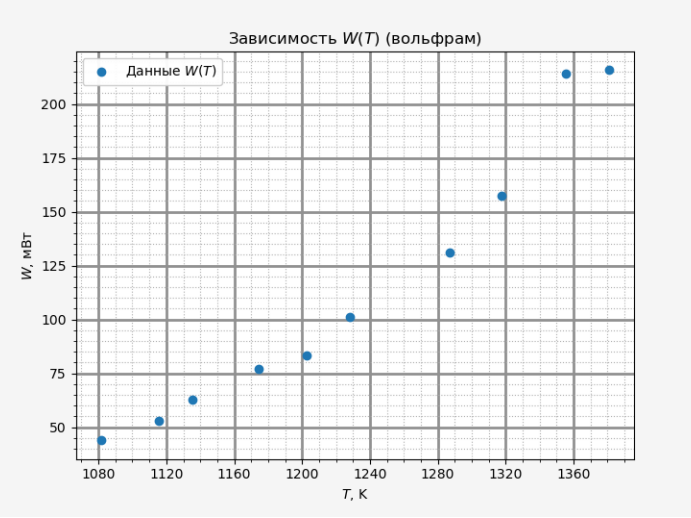
\includegraphics[width = 13 cm]{WT.png}
        \caption{График зависимости $W(T)$}
        \label{}
    \end{figure}

    \begin{figure}[h!]
        \centering
        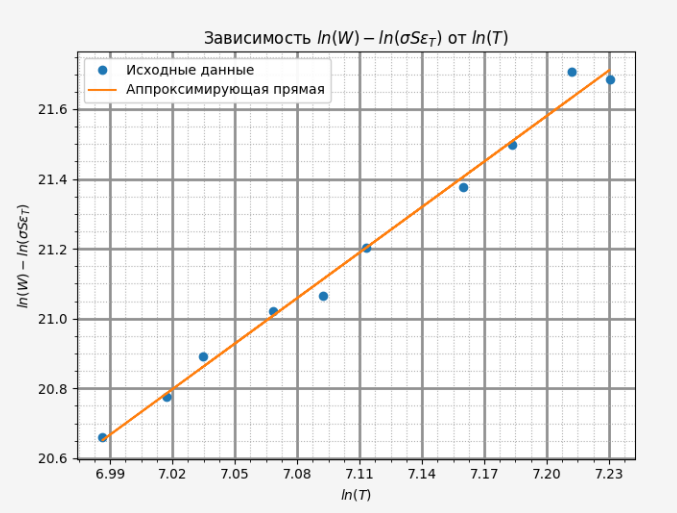
\includegraphics[width = 13 cm]{WT_log.png}
        \caption{График зависимости $W(T)$ в логарифмических осях}
        \label{}
    \end{figure}
    
    С помощью МНК измерим коэффициент из логарифмического графика $W(T)$:
    \begin{equation*}
        n = 4.34, \Delta n = 0.29, R^2 = 0.991
    \end{equation*}
    Полученное значение в рамках погрешностей сходится с теоретическим значением, равным 4 (закон Стефана-Больцмана).

    С учётом того, что для лампы накаливания $S = 5 \; \text{см}^2$, посчитаем для 3 различных температур ($T = 1174.45 \; K, T = 1380.63 \; K, T = 1081.73 K$) в рамках всего температурного диапазона значения постоянной Стефана-Больцмана (значения $\varepsilon_T$ посчитаны из таблицы):

    $$ \sigma_1 = (5.31 \pm 0.21) \cdot 10^{-9} \; \text{Вт} \cdot \text{м}^2 \cdot \text{К}^{-4} $$
    $$ \sigma_2 = (6.33 \pm 0.17) \cdot 10^{-9} \; \text{Вт} \cdot \text{м}^2 \cdot \text{К}^{-4} $$
    $$ \sigma_3 = (7.24 \pm 0.15) \cdot 10^{-9} \; \text{Вт} \cdot \text{м}^2 \cdot \text{К}^{-4} $$
    
    Полученные значения на порядок отличаются от теоретического значения постоянной Стефана-Больцмана.

\subsection{Измерение яркостной температуры неоновой лампочки}

    Термодинамическая температура неоновой лампочки примерно равна комнатной и не соответствует её яркостной температуре ($T_{\text{якр}} = \approx 828 ^\circ C$). Дело в том, что неоновая лампочка в принципе не является моделью абсолютно чёрного или серого тела, и её излучение носит совершенно другую природу (переход электронов между энергетическими уровнями). Неоновая лампа имеет похожую спектральную светимость при заданной длине волны $\lambda = 650$ нм, хотя её температура совсем не соответствует яркостной.


\section{Вывод}

    В результате работы проверена градуировка пирометра по АЧТ -- при значении, измеренном термопарой $(938 \pm 2) ^\circ C$, получены значения термодинамической температуры при убывании яркостной температуры во время измерений $(934 \pm 5) ^\circ C$ и при возрастании $(930 \pm 5) ^\circ C$. То есть значения, измеренные по пирометру, в рамках погрешностей совпадают со значением, измеренным термопарой.

    Для двух колец, изготовленных из различных материалов, зафиксировано различие яркостных температур при $\lambda = 650$ нм при одинаковых термодинамических температурах, т.к. различные материалы могут иметь различные зависимости спектральной светимости от длины волны.

    Подтверждена температурная зависимость закона Стефана-Больцмана для лампы накаливания (вольфрам) с результатами степени
    \begin{equation*}
        W \propto T^n, n = 4.34, \Delta n = 0.29, n_{th} = 4.
    \end{equation*}

    Во всём диапазоне измерений найдены постоянные Стефана-Больцмана для 3 различных температур $T = 1174.45 \; K, T = 1380.63 \; K, T = 1081.73 K$:
    $$ \sigma_1 = (5.31 \pm 0.21) \cdot 10^{-9} \; \text{Вт} \cdot \text{м}^2 \cdot \text{К}^{-4} $$
    $$ \sigma_2 = (6.33 \pm 0.17) \cdot 10^{-9} \; \text{Вт} \cdot \text{м}^2 \cdot \text{К}^{-4} $$
    $$ \sigma_3 = (7.24 \pm 0.15) \cdot 10^{-9} \; \text{Вт} \cdot \text{м}^2 \cdot \text{К}^{-4} $$
    Полученные значения отличаются на порядок от теоретического $\sigma = 5.67 \cdot 10^{-8} \; \text{Вт} \cdot \text{м}^2 \cdot \text{К}^{-4}$. Причины расхождения возможны из-за неверно заданной площади поверхности нитей лампы накаливания $S = 5 \; \text{см}^2$ (которая не влияет на поиск температурной зависимости $W(T)$), также возможны расхождения из-за того, что в рассчётах не учитываются потери на рассеивание тепла в окружающую среду (воздух).

    Для неоновой лампы измереноа яркостная температура $T_{\text{якр}} \approx 828 ^\circ C$ и проверено, что её термодинамическая темпаратура отличается от яркостной и примерно равна комнатной.


\begin{thebibliography}{9}
\bibitem{laba} 
Игошин Ф.Ф., Самарский Ю.А., Ципенюк Ю.М. 
\textit{Лабораторный практикум по общей физике: Учеб. пособие для вузов. Т. 3 Квантовая физика}. 
М.: Физматкнига, 2005.
\end{thebibliography}

\end{document}
